\chapter{Experiments}

This chapter presents the experiments. It is a crucial part of the thesis and has to dominate in the thesis. 
The experiments and their analysis should be done in the way commonly accepted in the scientific community (eg. benchmark datasets, cross validation of elaborated results, reproducibility and replicability of tests etc).


\section{Methodology}

\begin{itemize}
\item description of methodology of experiments
\item description of experimental framework (description of user interface of research applications – move to an appendix)
\end{itemize}


\section{Data sets}

\begin{itemize}
\item description of data sets
\end{itemize}


\section{Results}

\begin{itemize}
\item presentation of results, analysis and wide discussion of elaborated results, conclusions
\end{itemize}



\begin{table}
\centering
\caption{A caption of a table is \textbf{above} it.}
\label{id:tab:wyniki}
\begin{tabular}{rrrrrrrr}
\toprule
	         &                                     \multicolumn{7}{c}{method}                                      \\
	         \cmidrule{2-8}
	         &         &         &        \multicolumn{3}{c}{alg. 3}        & \multicolumn{2}{c}{alg. 4, $\gamma = 2$} \\
	         \cmidrule(r){4-6}\cmidrule(r){7-8}
	$\zeta$ &     alg. 1 &   alg. 2 & $\alpha= 1.5$ & $\alpha= 2$ & $\alpha= 3$ &   $\beta = 0.1$  &   $\beta = -0.1$ \\
\midrule
	       0 &  8.3250 & 1.45305 &       7.5791 &    14.8517 &    20.0028 & 1.16396 &                       1.1365 \\
	       5 &  0.6111 & 2.27126 &       6.9952 &    13.8560 &    18.6064 & 1.18659 &                       1.1630 \\
	      10 & 11.6126 & 2.69218 &       6.2520 &    12.5202 &    16.8278 & 1.23180 &                       1.2045 \\
	      15 &  0.5665 & 2.95046 &       5.7753 &    11.4588 &    15.4837 & 1.25131 &                       1.2614 \\
	      20 & 15.8728 & 3.07225 &       5.3071 &    10.3935 &    13.8738 & 1.25307 &                       1.2217 \\
	      25 &  0.9791 & 3.19034 &       5.4575 &     9.9533 &    13.0721 & 1.27104 &                       1.2640 \\
	      30 &  2.0228 & 3.27474 &       5.7461 &     9.7164 &    12.2637 & 1.33404 &                       1.3209 \\
	      35 & 13.4210 & 3.36086 &       6.6735 &    10.0442 &    12.0270 & 1.35385 &                       1.3059 \\
	      40 & 13.2226 & 3.36420 &       7.7248 &    10.4495 &    12.0379 & 1.34919 &                       1.2768 \\
	      45 & 12.8445 & 3.47436 &       8.5539 &    10.8552 &    12.2773 & 1.42303 &                       1.4362 \\
	      50 & 12.9245 & 3.58228 &       9.2702 &    11.2183 &    12.3990 & 1.40922 &                       1.3724 \\
\bottomrule
\end{tabular}
\end{table}  

\begin{figure}
\centering
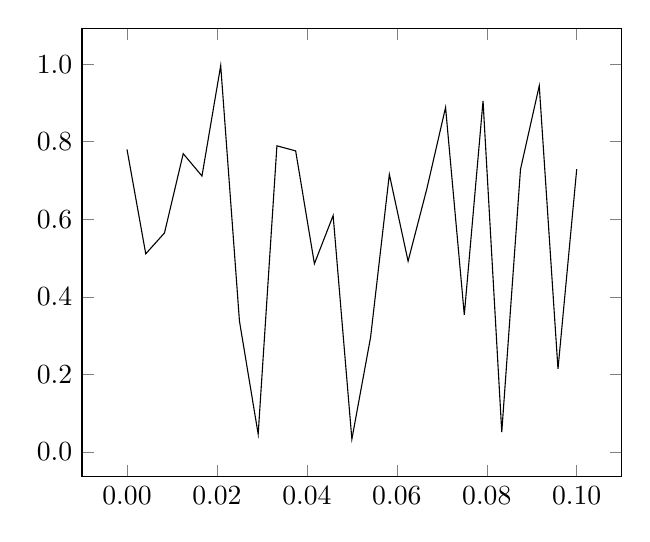
\begin{tikzpicture}
\begin{axis}[
    y tick label style={
        /pgf/number format/.cd,
            fixed,   % po zakomentowaniu os rzednych jest indeksowana wykladniczo
            fixed zerofill, % 1.0 zamiast 1
            precision=1,
        /tikz/.cd
    },
    x tick label style={
        /pgf/number format/.cd,
            fixed,
            fixed zerofill,
            precision=2,
        /tikz/.cd
    }
]
\addplot [domain=0.0:0.1] {rnd};
\end{axis} 
\end{tikzpicture}
\caption{Podpis rysunku po rysunkiem.}
\label{fig:2}
\end{figure}

